\documentclass{article}
\usepackage[utf8]{inputenc}

\usepackage[ruled, vlined,nofillcomment,linesnumbered]{algorithm2e}
\usepackage{cite}
\usepackage{url}
\usepackage{amsmath}
\usepackage{amssymb}
\usepackage{graphicx}
% \usepackage{subfig}
\usepackage[english]{babel}
\usepackage{booktabs}
\usepackage{nicefrac}
\usepackage{verbatim}
\usepackage{color}
\usepackage{float}
\usepackage{xspace}
\usepackage{mathtools}
\usepackage{etex}
\usepackage{natbib}
\usepackage{subcaption}
\usepackage{hyperref}
\usepackage{bbm}
\usepackage[nodayofweek]{datetime}

\usepackage{tikz,pgfplots,pgfplotstable}
\usetikzlibrary{positioning,fit,shapes}
\usetikzlibrary{decorations.pathreplacing}
\usetikzlibrary{arrows}

\DeclarePairedDelimiter\ceil{\lceil}{\rceil}
\DeclarePairedDelimiter\floor{\lfloor}{\rfloor}

\providecommand{\tightlist}{%
  \setlength{\itemsep}{0pt}\setlength{\parskip}{0pt}}

\newdateformat{mydate}{\shortmonthname[\THEMONTH] \twodigit{\THEDAY}{}, \THEYEAR}

\title{Example Solution for Assignment 1}
\author{}
\date{\mydate\today}


% \input{defines}

\begin{document}

\maketitle

\section{Question 1}\label{question-1}

(Credit to: Tuomo Tanila)

\subsection{Get all records with search key greater than 40}\label{section}

The tree nodes that must be fetched are: \textbf{I1}, \textbf{I2} as well as every node between \textbf{L2-L8} (that is \textbf{L2, L3, L4, L5, L6, L7} and \textbf{L8}). As we are searching all the records with search key greater than 40, we begin from the top node and choose the lower node that is between 30 and 80, that is \textbf{I2} in this case. After this we choose the node that is between 35 and 42. Finally we get to the leaf nodes and go all of them through.

\paragraph{common mistakes:}

\begin{itemize}
\tightlist
\item
  \textbf{I3} is visited (note that leaf nodes are doubly-linked) so \textbf{I3} is not visited
\end{itemize}


\subsection{Inserting a record with search key 88}\label{section-1}

As there is enough space for the key 88 in the tree, there is no need to additional operations (e.g. splitting leaves) after finding the correct leaf (\textbf{L6}). By inserting the search key \textbf{88*}, we will get the resulting tree in Figure~\ref{fig:q1-1}.

\begin{figure}[H]
  \centering
  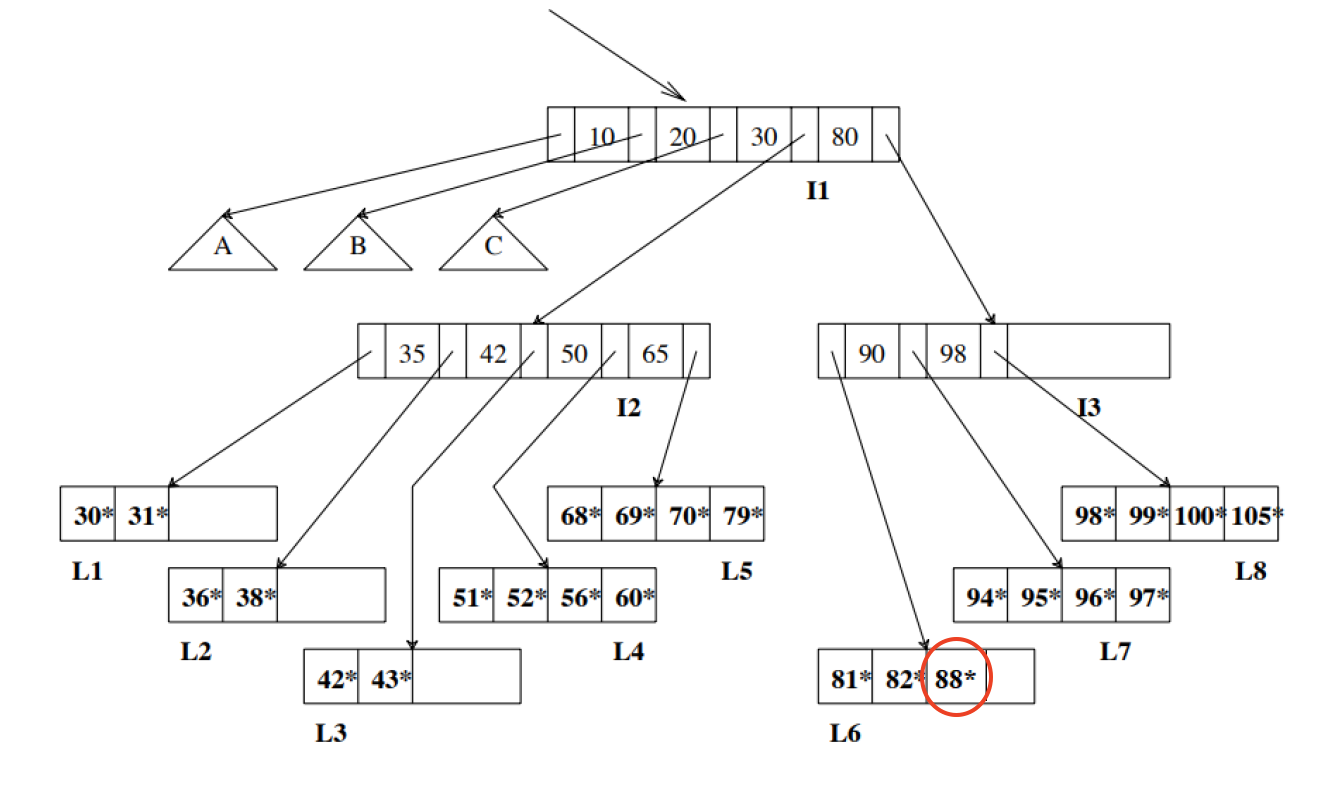
\includegraphics[width=0.9\linewidth]{figs/q1-2.png}
  \caption{B+ tree after inserting search key 88.}
  \label{fig:q1-1}
\end{figure}

\subsection{Inserting a record with search key 109}\label{section-2}

As there is not enough space for the key 109 in the tree, additional operations need to be performed.
The leaf \textbf{L8} will be split into two leaves so that we get a new one (\textbf{L9}).
The leaves are redistributed evenly and middle key is copied to the parent of L8. By inserting the search key \textbf{109*}, we will get the following tree in Figure~\ref{fig:q1-3}.

\begin{figure}[H]
  \centering
  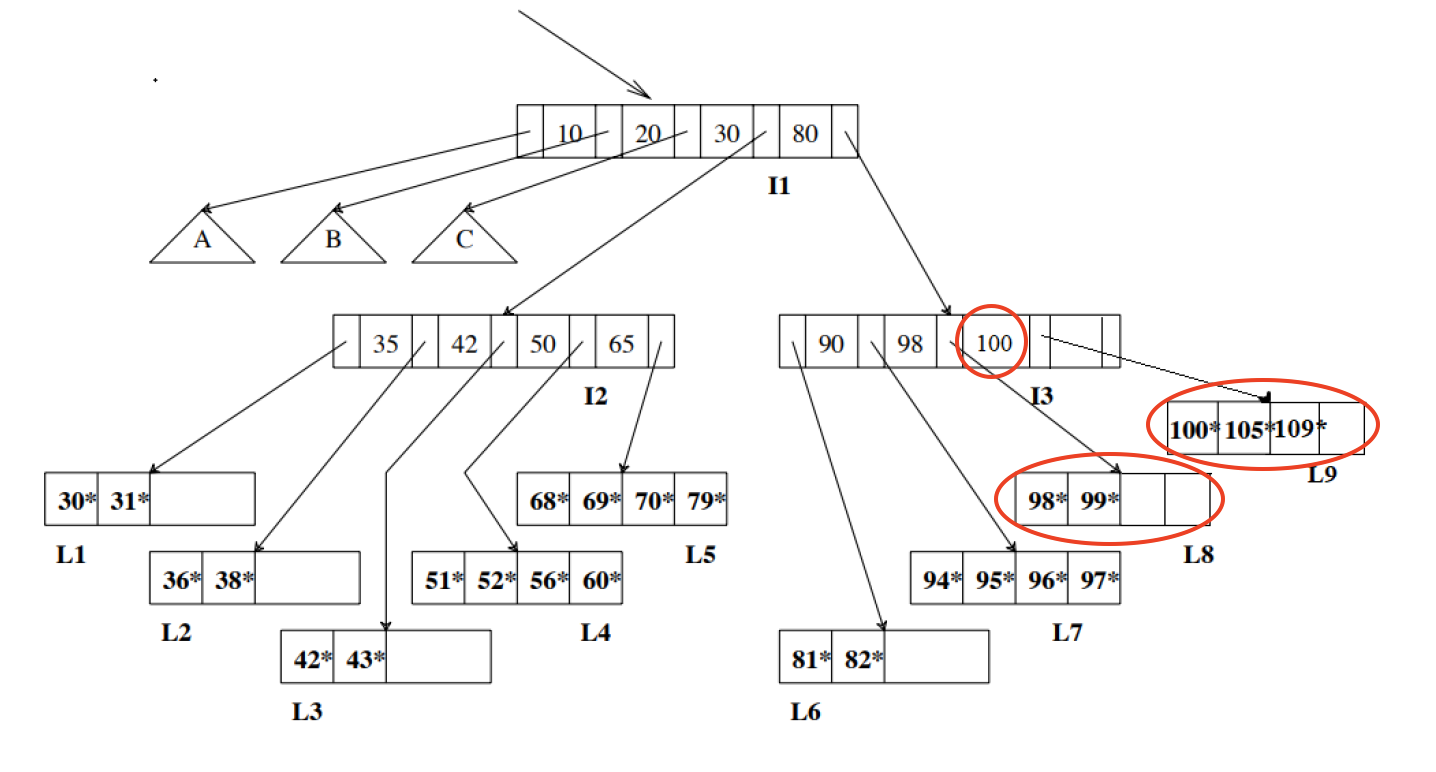
\includegraphics[width=0.9\linewidth]{figs/q1-3.png}
  \caption{B+ tree after inserting search key 109.}
  \label{fig:q1-3}
\end{figure}

\subsection{Contents and shape of subtrees A, B and C}\label{section-3}

\begin{itemize}
  \tightlist   
\item \textbf{tree height}: \textbf{A}, \textbf{B}, \textbf{C} should have the same height as \textbf{I2} and \textbf{I3}
\item \textbf{key range}: for A $[-\infty, 10)$, for B, $[10, 20)$, for C, $[20,30)$
\item \textbf{occupancy}:   each non-leaf node should have at least 2 search key values and 3 pointers while  each leaf node should have at least 2 data entries.
\end{itemize}
  
\section{Question 2}\label{question-2}

(Credit: Tuomo Tanila)

\subsection{Inserting 2}

We convert it to binary \textit{010} and it should be placed to \textbf{Bucket C}. This is shown in Figure~\ref{fig:q2-1}.

\begin{figure}[H]
  \centering
  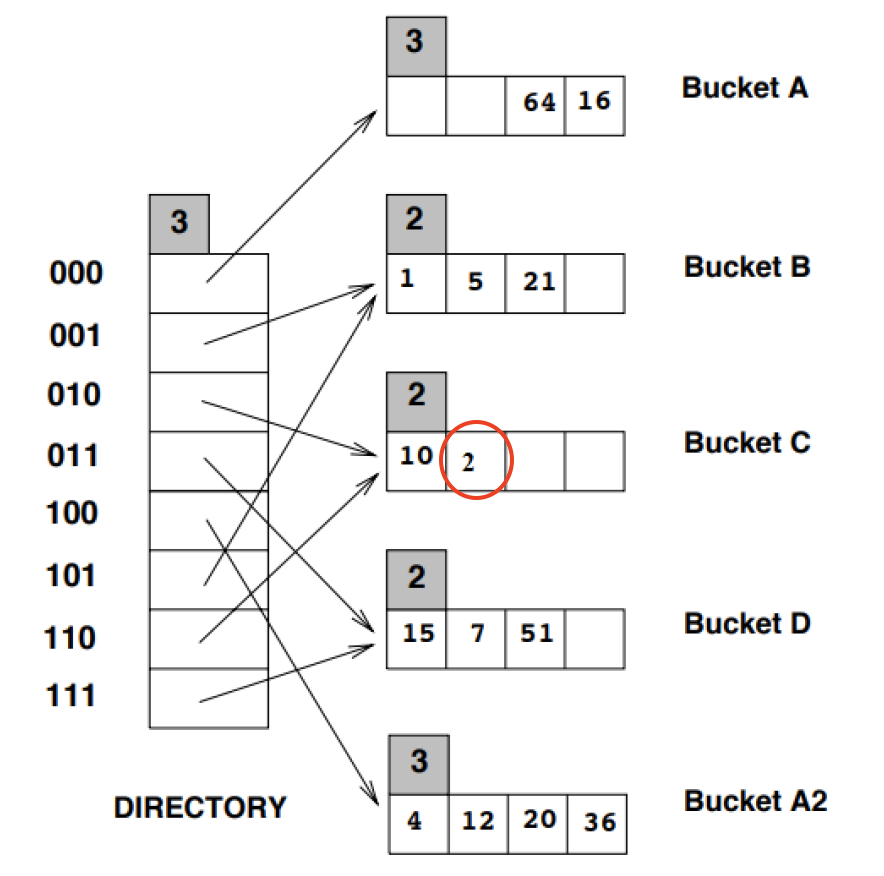
\includegraphics[width=0.9\linewidth]{figs/q2-1.png}
  \caption{Hash index after inserting 2}
  \label{fig:q2-1}
\end{figure}

\subsection{Inserting 25}

Similarly, its binary value is \textit{11001} and should be placed to \textbf{Bucket B}. This is shown in Figure~\ref{fig:q2-2}.

\begin{figure}[H]
  \centering
  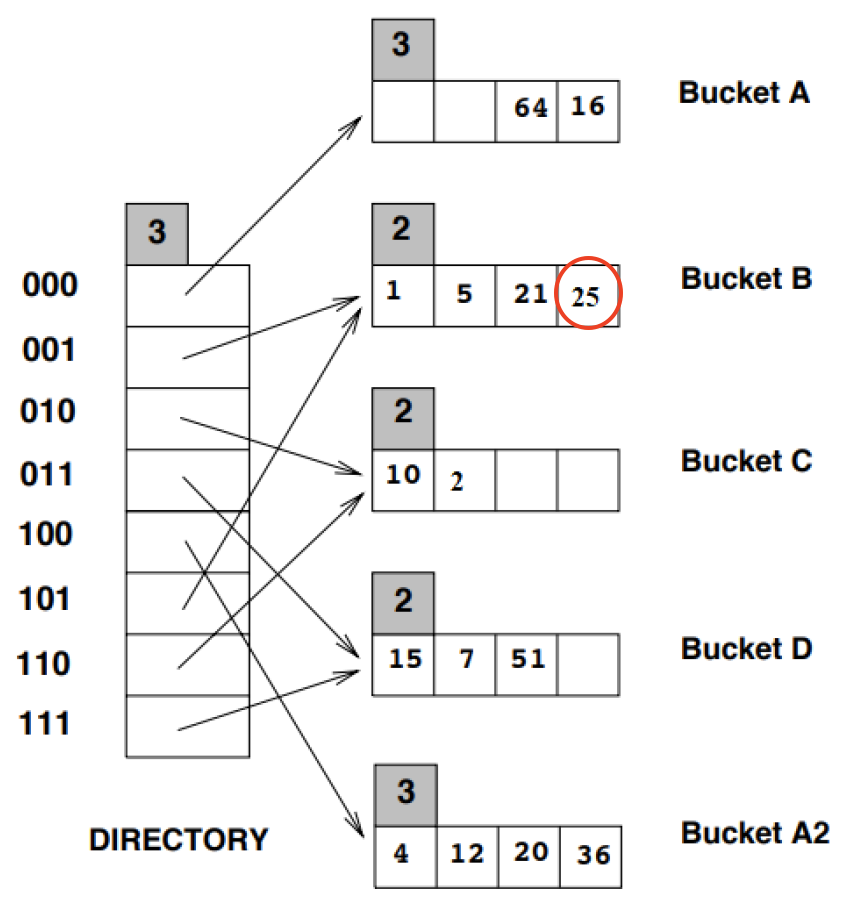
\includegraphics[width=0.9\linewidth]{figs/q2-2.png}
  \caption{Hash index after inserting 25}
  \label{fig:q2-2}
\end{figure}

\subsection{Inserting 0}

Similarly, its binary value is \textit{000} and should be placed to \textbf{Bucket A}.
This is shown in Figure~\ref{fig:q2-3}.

\begin{figure}[H]
  \centering
  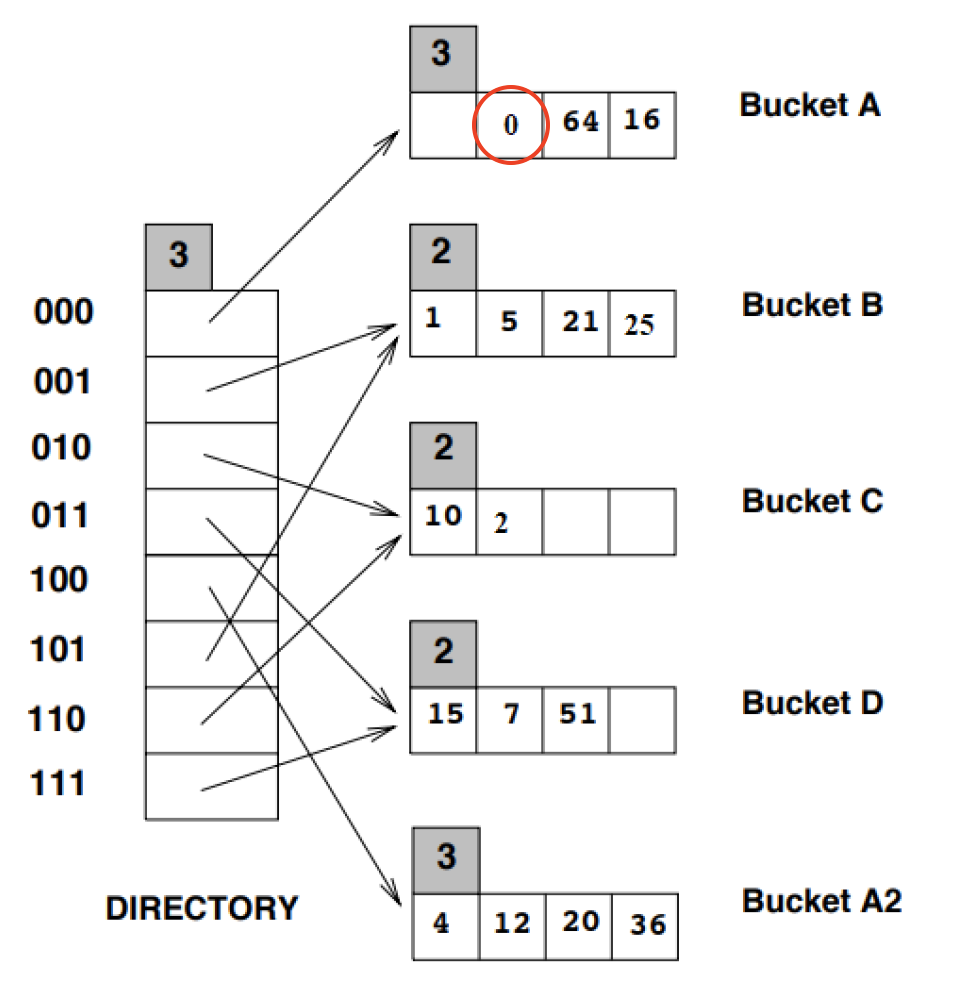
\includegraphics[width=0.9\linewidth]{figs/q2-3.png}
  \caption{Hash index after inserting 0}
  \label{fig:q2-3}
\end{figure}

\subsection{Inserting 31}

Similarly, its binary value is \textit{11111} and should be placed to \textbf{Bucket D}.
This is shown in Figure~\ref{fig:q2-4}.

\begin{figure}[H]
  \centering
  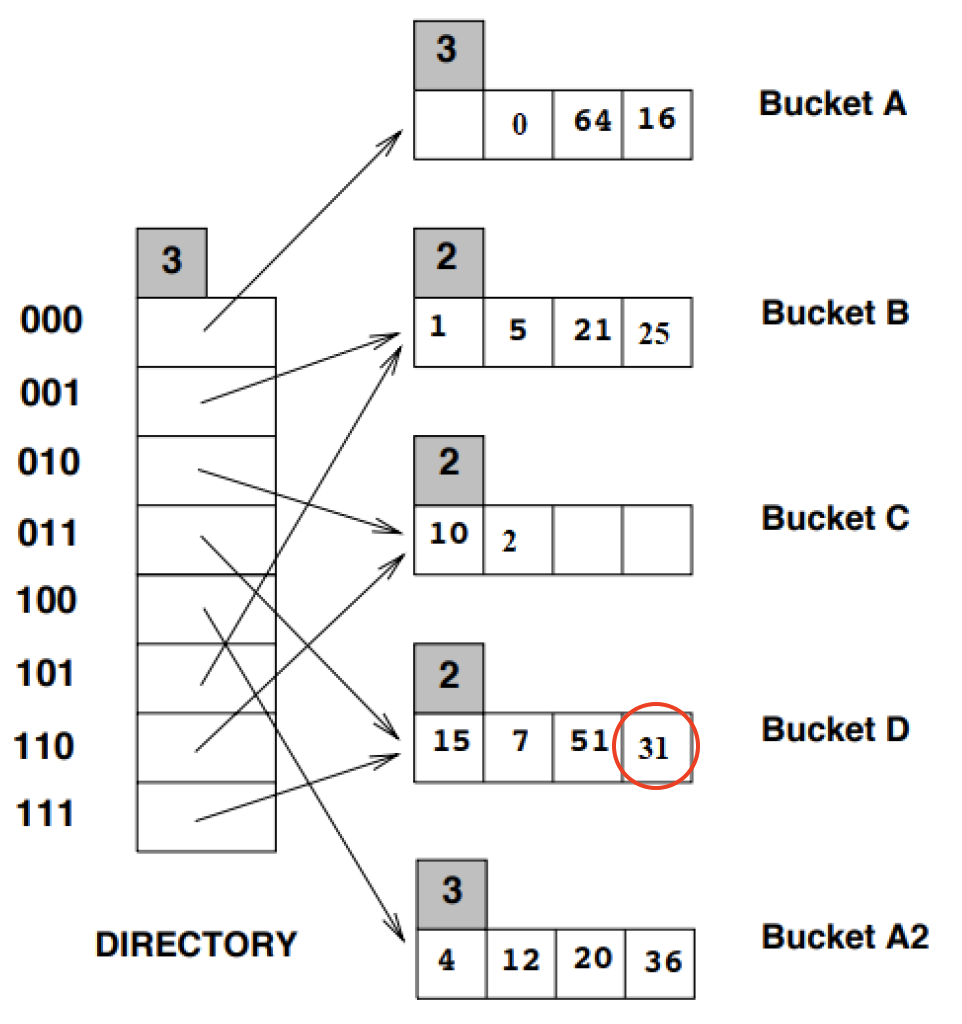
\includegraphics[width=0.9\linewidth]{figs/q2-4.png}
  \caption{Hash index after inserting 31}
  \label{fig:q2-4}
\end{figure}

\subsection{Inserting 68}

Finally, we need to split the bucket \textbf{A2} as there is no enough space for 68.
As a result, the new buckets have local depth 4 and The global depth is increased as well (now we take four least significant bits from binary numbers).
This is shown in Figure~\ref{fig:q2-5}.

\begin{figure}[H]
  \centering
  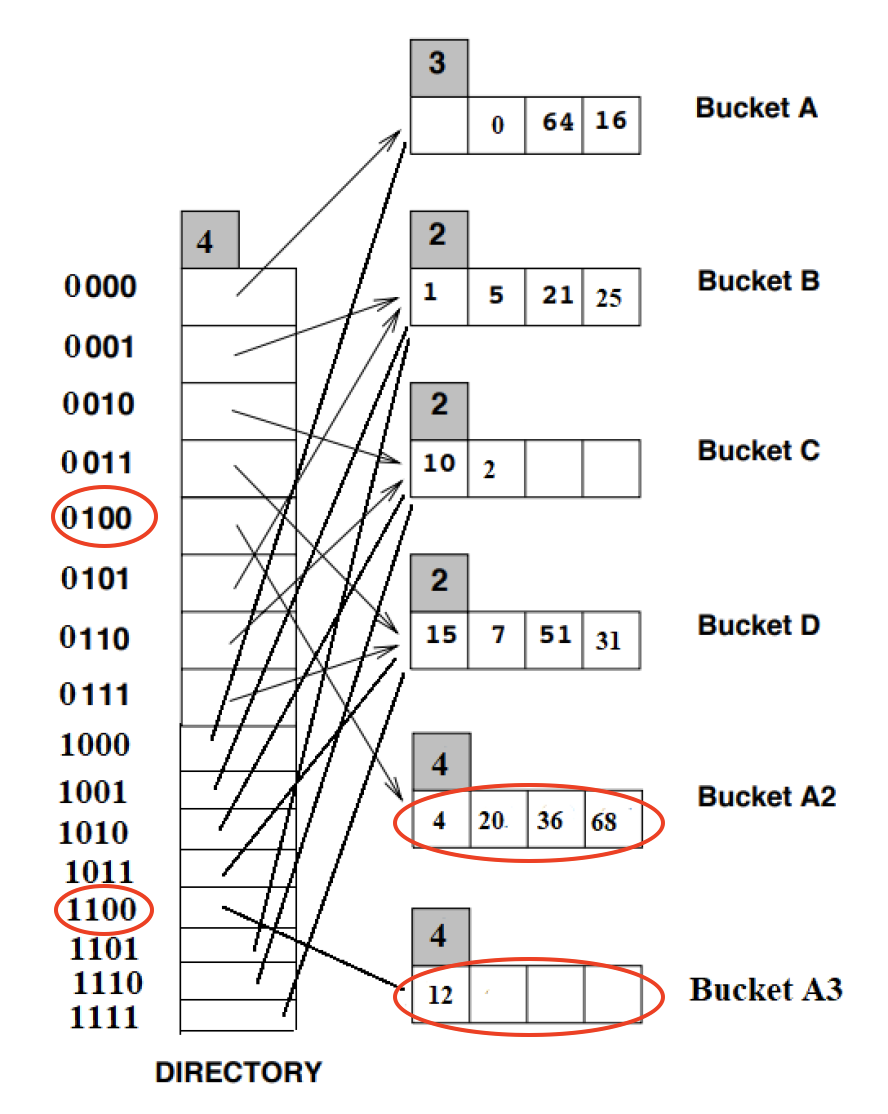
\includegraphics[width=0.9\linewidth]{figs/q2-5.png}
  \caption{Hash index after inserting 68.
    Bucket A2 is split into A2 and A3.
  Local depth on A2 and A3 as well as global depth increase to 4. }
  \label{fig:q2-5}
\end{figure}

\section{Question 3}\label{question-3}

\subsection{Via whole heap file}\label{via-whole-heap-file}

Because the heap files are unclustered/unordered, we need:

\[
  \frac{\text{number of all records}}{\text{number of records per page}} = \frac{10^6}{10} = 10^5
\]

\subsection{B+ tree index (alternative2)}\label{b-tree-index-alternative-2}

Denote
$\alpha$ as occupancy ratio of B+ tree,
$\beta$ as ratio of between size of one data entry and size of one record,
$F$ as the fan-out of the tree,
and $Q$ as the number of qualifying pages.

Then, we need

\[
  \log_F \frac{\beta}{\alpha} 10^5 + Q
\]

\subsection{Hash index (alternative 2)}\label{hash-index-alternative-2}

Again we use the notations from above, we need to use

\[
  \frac{\beta}{\alpha} 10^5 + Q
\]

\section{Question 4}\label{question-4}

\subsection{Number of runs in the first pass}

$\ceil{\frac{4000000}{17}} = 235295$

\subsection{Number of runs to sort completely}

$1 + \ceil{\log_{16} 235295} = 1 + \ceil{4.46} = 6$

\subsection{Total I/O cost}

$2 \times 4^6 \times 6 = 4.8 \times 10^7$

\subsection{Number of buffer pages needed to sort in exactly two passes}

Denote $B=17$ and $N=4\times 10^6$, we need to solve the following linear equation:

\[1 + \ceil{log_{B-1} \frac{N}{B}} = 2 \]

which  gives $N \approx 2000.5$. So we need at least 2001 buffer pages
\section{Question 5}\label{question-5}

Denote:

\begin{itemize}
\tightlist
\item
  $M=1000$ pages for R
\item
  $N=50$ pages for S
\item
  $B=52$ for number of buffer pages
\end{itemize}

\subsection{Page-oriented simple nested loops join}\label{page-oriented-simple-nested-loops-join}

If R is the outer loop, the cost is $M + M \times N = 51000$. 
And if S is the outer loop, the cost is $N + N \times M = 50050$. 

\subsection{Block nested loops join}\label{block-nested-loops-join}

If R is outer loop, then $M + \ceil{M / (B-2)} \times N = 2000$
If S is outer loop, then $N + \ceil{N / (B-2)} \times M = 1050$

\subsection{sort-merge join}\label{sort-merge-join}

For sorting on both R and S, the cost is:

\begin{itemize}
\tightlist
\item
  For R: $2 \times M \times (1 + \ceil{\log_{B-1}(\ceil{\frac{M}{B}})}) = 2 \times 1000 \times (1 + 1) = 4000$
\item
  For S: $2 \times N \times (1 + \ceil{\log_{B-1}(\ceil{\frac{N}{B}})}) = 2 \times 50 \times (1 + 0) = 100$
\end{itemize}

For merging, the cost is linear time, $M + N = 1050$

So in total, it costs 5150. 

\subsection{Hash join}\label{hash-join}

$3M+3N = 3150$






\bibliographystyle{plain}
\bibliography{references}
\end{document}


